\chapter{Proximity Based Authentication}
\label{proxAuth}
The emergence of the IoT is rapidly and drastically increasing the number of connected devices, posing new challenges towards solutions for authenticating this huge number of very heterogeneous  devices to their respective trust domains.
The enormous amount of data they create often contains privacy-sensitive information, which the users might prefer to not leak to a malicious party.
Moreover, the user would also prefer that no malicious device from an attacker joins his networks, and communicates with his devices.
In highly dynamic networks, devices frequently join or leave the network and occurs to secure interactions between entities that do not know each others a priori. 
Nevertheless, there are plenty of solutions which involve manual authentication but they are often not applicable in this kind of context.
In the users' everyday life can be involved many different devices, like smart light bulbs, air conditioning (HVAC) systems  \cite{Erickson2011OBSERVE:Energy} and different sensors, and in this case the user would have to repeat the authentication process for each device. 
Moreover, not all the devices are available for manual authentication due to the highly simplified hardware resources, lacking of user interface which makes then direct password entry or management  challenging or even impossible \cite{Jewell2015ConnectingInterfaces}.

As \acs{IoT} devices largely interact with their surroundings providing context-dependent functionalities, becomes important to include context into their access control mechanisms.
Due to the relation between context, proximity and trust \cite{Pitelis2013LocalProximity}, exploiting common contextual features among communicating devices to generate a security scheme might provide a sense of security similar to the one perceived as natural by individuals.
Avoiding to involve users in the protocol (e.g., typing in a password) and other \textit{human-in-the-loop} solutions would then reduce the number of human errors related to security and the users' burden.

Authentication usually takes the form of a challenge-response mechanism whereby a verifier party $\mathcal{V}$ verify the possession of a pre-shared key \textit{K}  with a prover party $\mathcal{P}$ by encrypting or authenticating a random challenge (using \textit{K}) sent by $\mathcal{P}$.

\section{Context Data Collection}
The goal of our experiment was to collect a comprehensive real-world dataset of ambient information that can serve as a baseline for analyzing a zero-interaction authentication scheme. 
We propose two scenarios where we collected data using  \textit{Raspberry Pi 3}. 
Audio data was collected using a USB sound card with mini microphone, which recorded a mono audio stream with a 44.1 kHz sampling rate, and encoded it using the MP3 format. 
The Raspberry Pi also collected with a frequency of one sample every 10 seconds the following context information:
\begin{itemize}
    \item \textbf{temperature}, \textbf{humidity}, \textbf{barometric pressure} using Adafruit BME280 sensor which offers measures of humidity with $ \pm 3 \%$ accuracy, barometric pressure with $\pm 1 hPa$ absolute accuracy, and temperature with $\pm 1.0°C $ accuracy;
    \item \textbf{digital light}: using Adafruit TSL2591 high dynamic range digital light sensor, allowing for exact lux calculations and can be configured for different gain/timing ranges to detect light ranges from up to $188uLux$ up to $88,000$ Lux on the fly;
    \item \textbf{vibration}: using the MPU6050 accelerometer and gyroscope. offering a user-programmable gyroscope full-scale  range of  $\pm 250$, $\pm 500$, $\pm 1000$ and $\pm 2000°/sec $ and a user-programmable accelerometer full-scale range of $\pm 2g$, $\pm 4g$, $\pm 8g$ and $\pm 16g$.
\end{itemize}



 
\subsection{Scenario 1: Office Environment}
In our first case-study, we position the devices in an office environment. 
Ambient audio was originated from individuals outside of the office room and from a computer located close to the devices. 
The context information are collected for 12 hours and the the devices are collocated close to each others.

\subsection{Scenario 2: Factory Environment}
Another typical application for IoT devices is the deployment in industrial environment.
In our second case-study, we position the devices in a factory environment. 
Ambient audio was originated loud machines and people working.
The context information are collected for 24 hours during the week, resulting then in hours with people working and hours where the ambient audio is only from the machines.
Four devices were playing the role of co-located devices and they positioned 1 meter of distance between each others. Three other devices were located 6 meters, 12 meters and 35 meters away from that group. 
The summary of device locations in the factory scenario is given in Figure \ref{fig_devices_loacation}.

\begin{figure}[!h]
\centering
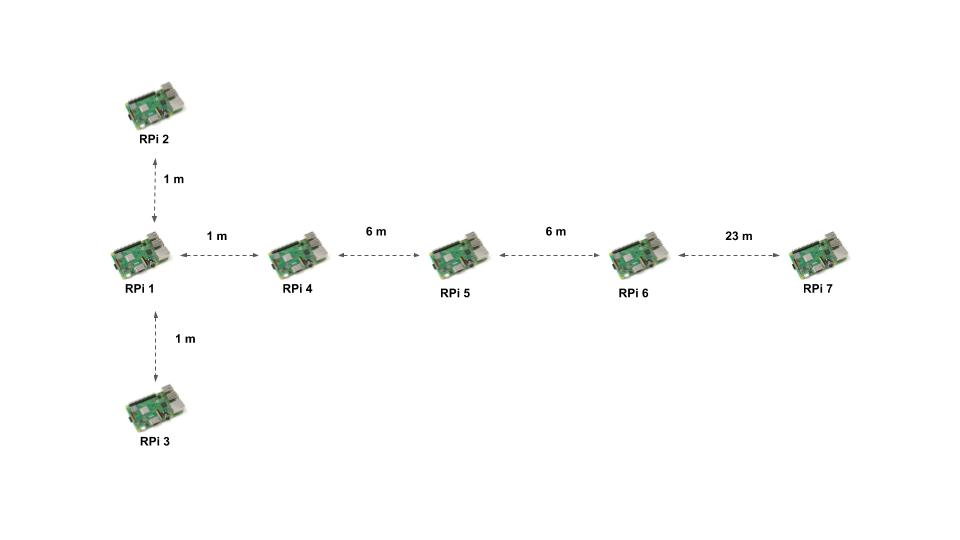
\includegraphics[width=6.5in]{images/devices_location.jpg}
\caption{Distance between each device in the factory environment.}
\label{fig_devices_loacation}
\end{figure}

\section{Adversary Model}
We assume a standard Dolev-Yao adversary model \cite{Dolev1981OriginalProtocols} where the adversary has complete control over all communication channels and it is not able to compromise the nodes. 
The adversary model considered for the design of a context-based authentication scheme is shown in Figure \ref{fig_environmentAttack}.
The model shows a network of devices located in the same environment, such as an office or in a delimited area in an industry, in which the devices are able to get the same ambient data such as light, audio and humidity. 
The goal of the adversary is to carry out relay attack by convincing the other nodes that it is nearby when in fact it is far away. 
The proposed countermeasure against relay attack which is based on the natural  assumption  that  two  entities  will  sense  similar ambient environments when they are co-present.
\begin{figure}[!h]
\centering
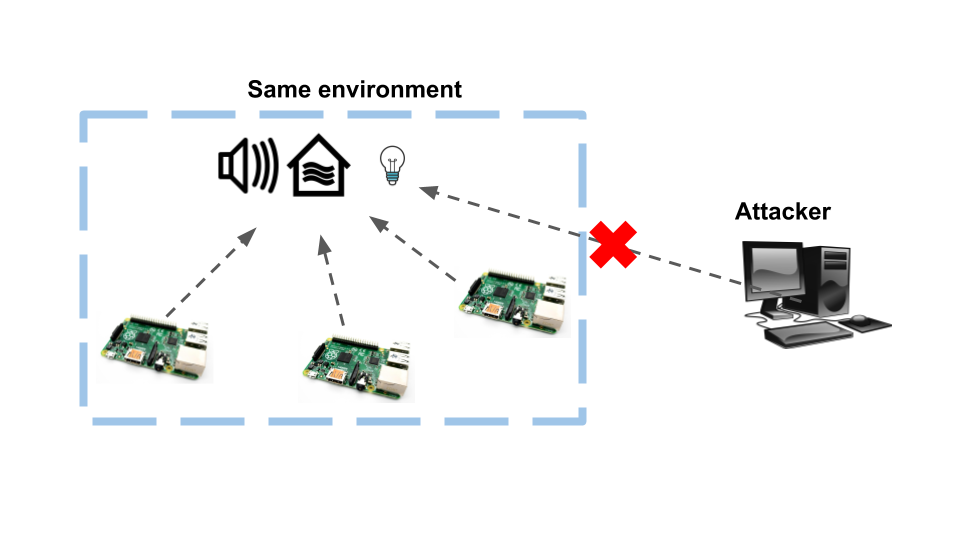
\includegraphics[width=5in]{images/environmentAttack.png}
\caption{For an attacker it is not possible to acquire the data from the user environment such as ambient sound, temperature and light.}
\label{fig_environmentAttack}
\end{figure}